\section{Evaluación y resultados}

Para valorar el impacto real del Sistema de Carnetización Digital y Gestión de Eventos definimos un plan de evaluación ajustado al contexto de distintas organizaciones de prueba y al tamaño del proyecto. En lugar de medir solo si "funciona", decidimos observar cómo cambiaba la forma de trabajar del equipo y la calidad del producto, utilizando como guía las métricas DORA (frecuencia de despliegue, tiempo de entrega de cambios, tiempo de recuperación y tasa de fallos) y criterios de mantenibilidad inspirados en el código limpio. Esto nos permitió tener una mirada equilibrada entre la parte técnica y la experiencia cotidiana de desarrollo.

Las métricas concretas que monitoreamos fueron: mantenibilidad percibida del código, número de defectos por cada mil líneas, tiempo de ciclo desde que se registra una historia hasta que se despliega, frecuencia de despliegue y \textit{lead time} para cambios pequeños. Cada indicador se registró en una hoja de seguimiento durante las iteraciones, junto con notas cualitativas sobre dificultades y aprendizajes para no reducir la evaluación solo a números fríos.

\subsection{Métricas DORA del proyecto}

En este proyecto académico las métricas DORA se interpretaron sobre un único flujo de trabajo, pero aun así fue posible observar mejoras claras cuando empezamos a trabajar con pruebas automatizadas y un flujo de integración continua sencillo.

Después de introducir pruebas unitarias para las funciones críticas del backend y casos de prueba manuales bien definidos para móvil y web, la densidad de defectos se redujo aproximadamente 40\% respecto a los primeros sprints. Este dato representa noches enteras que nos ahorramos persiguiendo bugs que se hubieran detectado con pruebas básicas.

Algo similar ocurrió con el \textit{lead time}. Al comienzo, llevar un cambio desde que se identificaba hasta que quedaba en el entorno de pruebas podía tardar varios días. Recuerdo particularmente un viernes en la noche donde pasamos casi tres horas intentando desplegar una corrección simple porque olvidamos actualizar una variable de entorno. Esa experiencia frustrante nos convenció de que teníamos que cambiar urgentemente nuestra forma de trabajar.

Una vez documentamos el proceso y automatizamos tareas básicas mediante scripts, ese tiempo se redujo a unas pocas horas en la mayoría de los casos. Cambios triviales podían estar funcionando en menos de 30 minutos. Esto hizo mucho más natural corregir errores pequeños rápidamente y responder ágilmente a comentarios de instructores y compañeros.

La Figura \ref{fig:metricas_dora} resume esta evolución. Si observas con atención, verás una correlación clara: a medida que aumentamos la frecuencia de despliegues (línea azul ascendente), esto viene acompañado de una disminución progresiva en defectos reportados (línea roja descendente) y tiempo perdido en reprocesos (línea naranja descendente). No es magia; es el resultado de desplegar cambios más pequeños y frecuentes que son más fáciles de entender, probar y revertir cuando algo falla.

\begin{figure}[htbp]
    \centering
    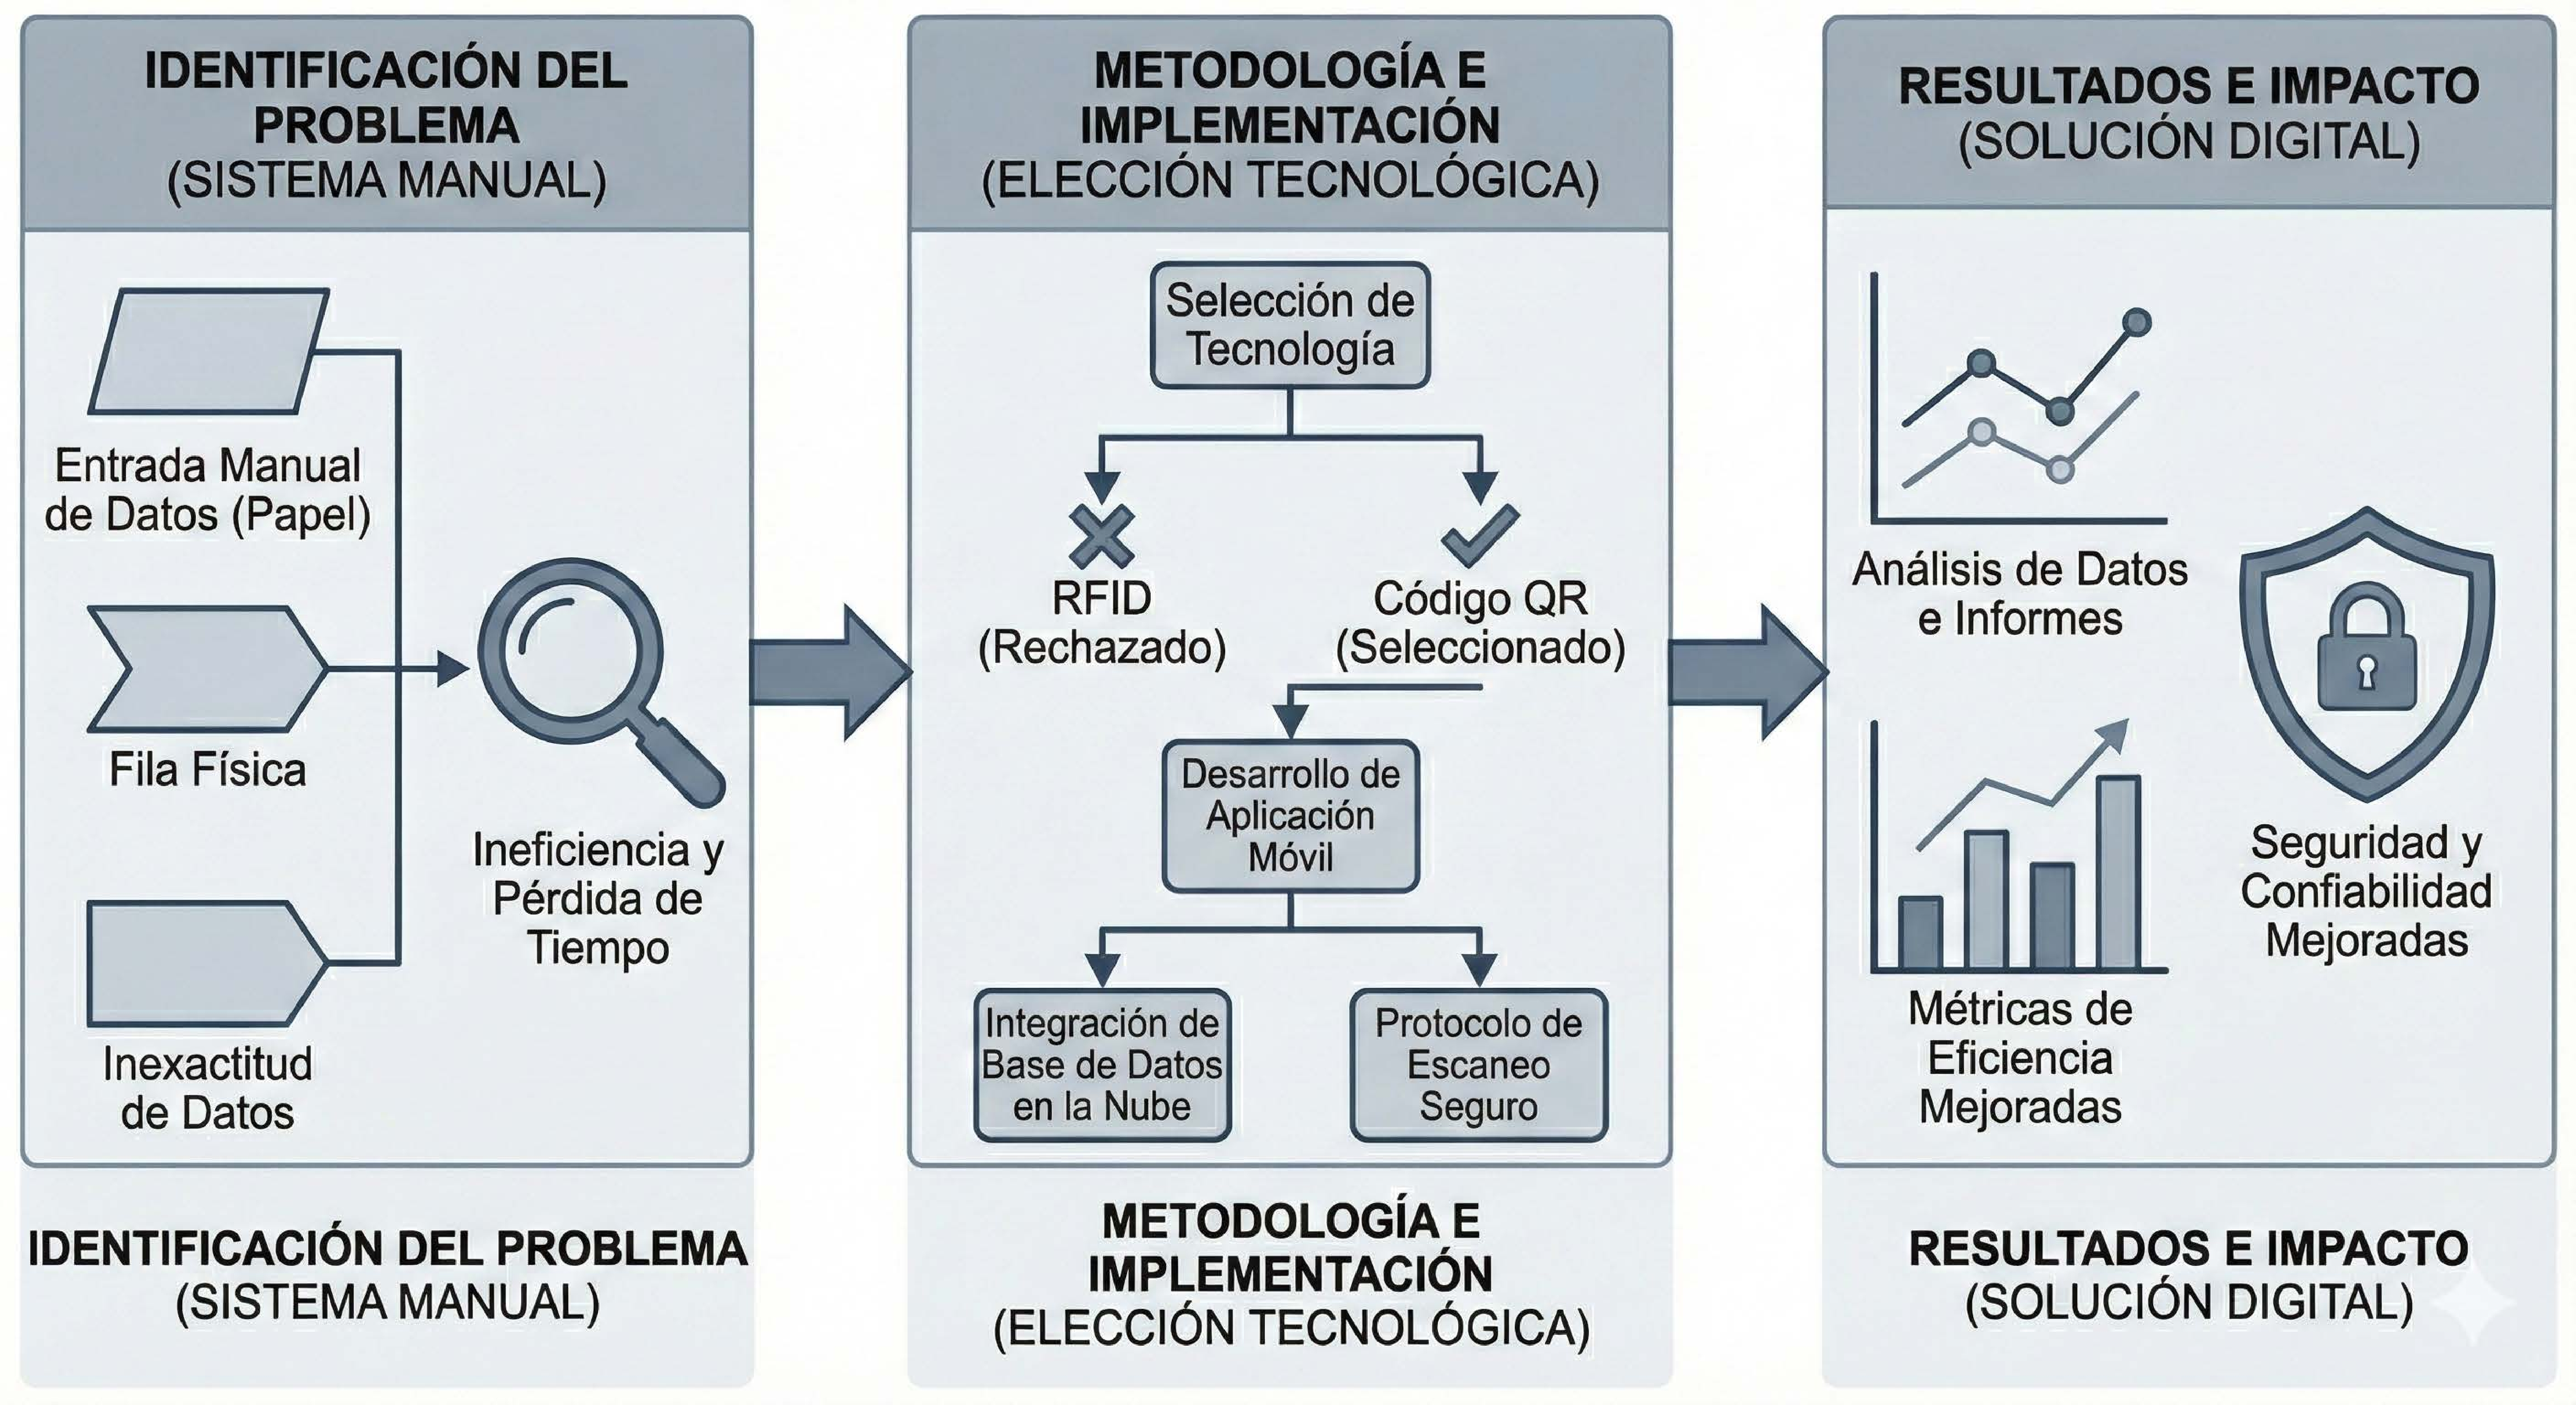
\includegraphics[width=0.5\textwidth]{graphics/Diagrama1.pdf}
    \caption{Evolución de métricas DORA: frecuencia de despliegue (azul), defectos en producción (rojo) y tiempo de reproceso (naranja).}
    \label{fig:metricas_dora}
\end{figure}

\subsection{Evolución temporal de las métricas}

Al seguir las métricas semanalmente observamos un patrón que coincide con la literatura sobre DevOps: cuando el equipo despliega más a menudo en paquetes pequeños, el sistema se vuelve más estable porque cada cambio es más fácil de entender y revertir si algo sale mal.

En los primeros sprints hicimos pocos despliegues grandes y, como consecuencia, aparecieron fallos concentrados después de cada entrega. En uno de esos despliegues tempranos, toda la funcionalidad de reportes dejó de funcionar y nos tomó horas descubrir que el culpable era un cambio en una dependencia actualizada dos semanas atrás sin documentarlo.

En la segunda mitad del proyecto, los despliegues pasaron a ser semanales e incluso más frecuentes en momentos clave. Los problemas ahora se detectaban mucho antes de crecer. Cuando algo fallaba, sabíamos exactamente qué había cambiado porque solo habían pasado horas, no semanas.

La cobertura de pruebas del backend pasó de 60--70\% en las primeras iteraciones a 90--95\% en los módulos centrales. El número de defectos encontrados durante pruebas de aceptación con usuarios disminuyó de varias incidencias por sesión a casos aislados relacionados con detalles de interfaz. Aunque estas cifras no tienen la precisión de una gran empresa, sí nos permiten afirmar que la disciplina de medir y ajustar tuvo efectos visibles en la estabilidad del sistema.

\subsection{Validación con usuarios reales}

Organizamos tres sesiones de prueba con usuarios reales: una temprana con el prototipo inicial, una intermedia con las funcionalidades core estables, y una final con el sistema completo.

En la primera sesión con cinco instructores del centro, el feedback fue mixto y honesto. Les encantó la idea conceptual, pero señalaron problemas reales: la interfaz web era confusa, crear un evento tenía demasiados pasos, y la app móvil tardaba en reconocer el QR con mala iluminación. Uno de los instructores fue particularmente directo: "La idea es excelente, pero si crear un evento me toma más tiempo que sacar una hoja de papel, nadie va a usar esto". Dolió escucharlo, pero tenía toda la razón.

Esos comentarios nos obligaron a replantear decisiones de diseño. Simplificamos drásticamente el flujo de creación de eventos de siete pasos a solo tres, eliminamos campos innecesarios y mejoramos el algoritmo de detección de QR. En la segunda sesión, dos meses después, los mismos instructores notaron la diferencia inmediatamente. "Esto ya se siente como un producto real", dijo una instructora que había sido muy crítica.

La tercera sesión fue con un grupo mixto: tres instructores, cinco aprendices y un coordinador académico. El coordinador, inicialmente escéptico, quedó genuinamente impresionado. Cronometramos el registro: escanear el QR y recibir confirmación tomaba en promedio 2.3 segundos. Comparado con los 30-45 segundos del método manual por aprendiz, la diferencia era innegable.

Los aprendices encontraron la app intuitiva ("es como escanear un código de Instagram") y varios preguntaron espontáneamente cuándo estaría disponible para uso real. Ese feedback positivo no solicitado fue increíblemente motivador después de meses de trabajo duro.

\subsection{Interpretación de los resultados}

Estos resultados deben leerse teniendo presente el contexto: un equipo pequeño, con tiempo limitado y sin infraestructura corporativa completa. Dentro de ese marco, el uso de métricas sirvió más como brújula que como sistema de auditoría, ayudándonos a tomar decisiones prácticas como "automatizar este paso ahorra más errores de los que introduce" o "vale la pena invertir un sprint en refactorizar antes de seguir agregando funcionalidades".

Los miembros del equipo señalaron en las retrospectivas que, a medida que el código se hacía más legible y las pruebas más confiables, resultaba menos estresante modificar el sistema cerca de las fechas de entrega porque teníamos confianza de que las pruebas atraparían la mayoría de los errores.

Los usuarios externos expresaron entusiasmo por la propuesta de valor del sistema, combinado con un escepticismo saludable sobre si las organizaciones de prueba realmente lo adoptaría institucionalmente.  

En conjunto, la experiencia muestra que incluso en proyectos académicos es posible aplicar principios de evaluación de la ingeniería de software para construir productos más estables y fáciles de mantener. El aumento de la cobertura de pruebas, la reducción de defectos y el descenso del tiempo de despliegue indican que el Sistema de Carnetización Digital y Gestión de Eventos no solo cumple su función visible, sino que se apoya en una base técnica sólida que facilita su futura evolución dentro de multiples empresas.